%This work is licensed under the Creative Commons License Attribution 4.0 International (CC-BY 4.0)
%https://creativecommons.org/licenses/by/4.0/legalcode
\documentclass[rgb]{standalone}
\usepackage{tkz-euclide}
\definecolor{myorange}{hsb}{0.0833, 1, 0.8}
\definecolor{mygreen}{hsb}{0.3333, 1, 0.8}
\definecolor{myblue}{hsb}{0.5833, 1, 0.8}
\definecolor{mymagenta}{hsb}{0.8333, 1, 0.8}
\begin{document}
	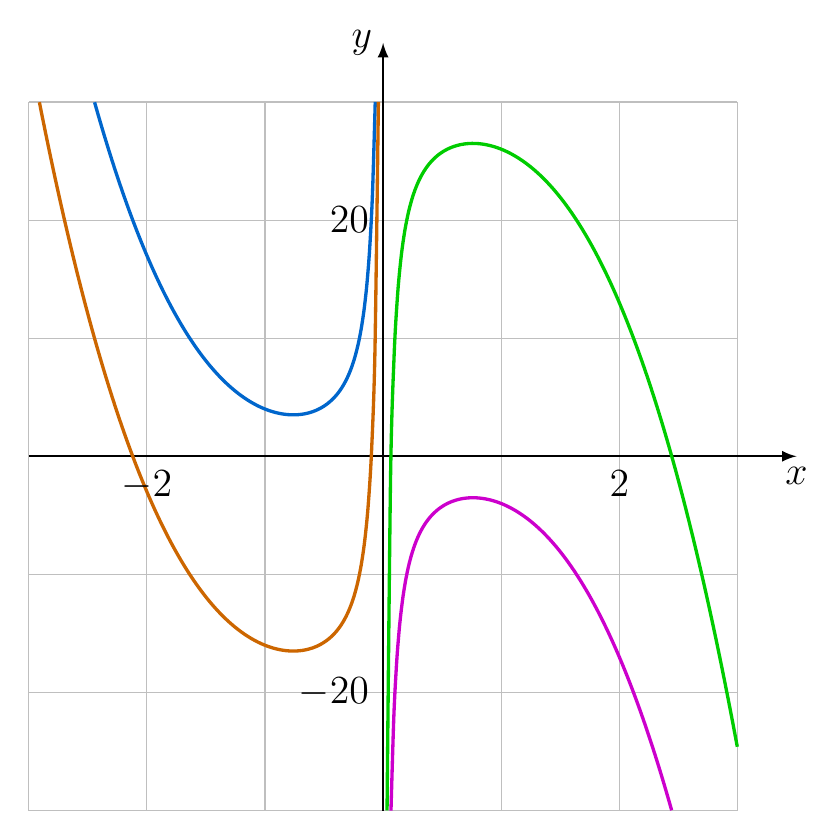
\begin{tikzpicture}[scale=1.5, font=\Large]
		% Coordinate system
		\tkzInit[xmin=-3,xmax=3,ymin=-3,ymax=3]
		\tkzGrid[color=lightgray]
		\tkzDrawX[thick]
		\tkzDrawY[thick]	
		\draw[very thick,domain=-0.066668:-2.44358, smooth,samples=100,variable=\x,myblue] plot ({\x}, {-0.2/\x-0.2*\x*\x*\x});	
		\draw[very thick,domain=-0.04:-2.91056, smooth, samples=100,variable=\x,myorange] plot ({\x}, {-0.2/\x-0.2*\x*\x*\x-2});	
		\draw[very thick,domain=0.0333334:3, smooth, samples=100,variable=\x,mygreen] plot ({\x}, {-0.2/\x-0.2*\x*\x*\x+3});	
		\draw[very thick,domain=0.066668:2.44358, smooth,samples=100,variable=\x,mymagenta] plot ({\x}, {-0.2/\x-0.2*\x*\x*\x});		
		% Labels
		\node[below=0.5mm] at (-2,0){$-2$};
		\node[below=0.5mm] at (2,0){$2$};
		\node[left=0.5mm] at (0,-2){$-20$};
		\node[left=0.5mm] at (0,2){$20$};
	\end{tikzpicture}	
\end{document}